\documentclass[11pt]{article}
\usepackage[margin=1in]{geometry}
\usepackage{graphicx}
\usepackage{amsmath,amssymb}
\usepackage{booktabs}
\usepackage[numbers,sort&compress]{natbib}  % MRM: numbered (Vancouver) references
\usepackage{xcolor}
\usepackage[colorlinks=true,linkcolor=blue,citecolor=blue,urlcolor=blue]{hyperref}
\usepackage{microtype}
\usepackage{caption}
\emergencystretch=2em

\newcommand{\Dstar}{D^{*}}
\newcommand{\unit}[1]{\,\mathrm{#1}}

\title{\textbf{Gauge: Distribution-Free Conformal Coverage for IVIM Parameter
Maps, and the Identifiability Wall in the Pseudo-Diffusion Compartment}}
\author{Avery Karlin\\[2pt]
\small ORCID: \href{https://orcid.org/0000-0003-3848-6782}{0000-0003-3848-6782}}
\date{}

\begin{document}
\maketitle

\begin{abstract}
\noindent
\textbf{Purpose:} To bring distribution-free conformal prediction to intravoxel
incoherent motion (IVIM) parameter mapping, benchmark it against model-based
uncertainty quantification (UQ), and test whether its advantage concentrates in
the ill-posed pseudo-diffusion compartment $\Dstar$.

\noindent
\textbf{Methods:} On a controlled, seeded synthetic cohort built from our own
bi-exponential forward model with Rician noise, we compare split-conformal and
conformalized quantile regression (CQR) against four model-based baselines
(probabilistic neural network, mixture-density deep ensemble, deep ensemble,
per-voxel Bayesian MCMC), measuring marginal and (SNR $\times$
true-$\Dstar$-tercile) conditional coverage and sharpness. A
Fisher-information / Cram\'er--Rao analysis diagnoses the residual gap; weighted
(nonexchangeable) conformal and a label-free deployment monitor stress
exchangeability; a qualitative in-vivo demonstration is included.

\noindent
\textbf{Results:} Model-based IVIM UQ is overconfident \emph{broadly} across $D$,
$\Dstar$, and $f$ (not specifically pseudo-diffusion), so the naive marginal
hypothesis is rejected. Conformal and conformalized methods restore near-nominal
marginal coverage everywhere ($|\text{gap}|\le 0.024$), and conformalizing the MDN
is the sharpest valid recipe ($0.65$--$0.79\times$ pure-CQR width). The real
failure is conditional: the high-$\Dstar$ regime under-covers for every method at
every SNR, and no label-free method closes the gap because the Cram\'er--Rao bound
on $\Dstar$ reaches the regime-bin width -- an irreducible identifiability limit.
The wall is robust to the b-value scheme; weighted conformal recovers covariate
shift but not forward-model misspecification; the monitor fires before coverage
fails but is blind to the latent gap.

\noindent
\textbf{Conclusion:} Conformal prediction supplies the finite-sample coverage
guarantee model-based IVIM UQ lacks, and conformalizing a strong base is sharpest.
The high-$\Dstar$ compartment is an identifiability limit we characterize, not
solve.
\end{abstract}

\vspace{0.5em}
\noindent\textbf{Keywords:} intravoxel incoherent motion (IVIM); uncertainty
quantification; conformal prediction; identifiability; pseudo-diffusion;
quantitative MRI.

\section{Introduction}
IVIM imaging~\citep{lebihan1988} separates microcirculatory perfusion from tissue
diffusion by fitting the bi-exponential signal
\begin{equation}
\frac{S(b)}{S_0} = f\,e^{-b\Dstar} + (1-f)\,e^{-bD},
\label{eq:ivim}
\end{equation}
where $b$ is the diffusion weighting (s/mm$^2$), $D$ the tissue diffusion
coefficient, $\Dstar \gg D$ the pseudo-diffusion coefficient, and $f$ the
perfusion fraction. Equation~\eqref{eq:ivim} is notoriously ill-posed: $\Dstar$ is
poorly constrained because the fast-decaying perfusion term contributes only at
low $b$, and small perfusion fractions make it nearly unidentifiable. Clinical use
of IVIM parameter maps therefore demands trustworthy \emph{per-voxel uncertainty},
not just point estimates.

The dominant approach to IVIM UQ is \emph{model-based}: probabilistic neural
networks, deep ensembles, mixture-density networks, and Bayesian fitting place a
distribution over parameters and read intervals from it. These methods make
distributional assumptions and carry \emph{no finite-sample coverage guarantee};
the most comprehensive IVIM-UQ study to date~\citep{casali2026} documents that
such models are well-calibrated for $D$ and $f$ but \emph{overconfident in
$\Dstar$}. \emph{Conformal prediction}~\citep{vovk2005,lei2018,angelopoulos2023}
offers the complementary property: under exchangeability of calibration and test
data, it produces intervals with finite-sample, distribution-free marginal
coverage for \emph{any} base predictor -- a biased base only widens the interval,
it does not break coverage. Conformalized quantile regression
(CQR)~\citep{romano2019} makes these intervals input-adaptive. Conformal UQ has
been applied to quantitative MRI relaxometry and field
mapping~\citep{birk2024}, but never to the ill-posed IVIM inverse problem, and
never benchmarked head-to-head against model-based IVIM UQ.

This paper closes that gap and, in doing so, \emph{reframes} the question. We began
with the hypothesis that conformal prediction's advantage would concentrate in the
unstable $\Dstar$ (and secondarily $f$) compartment, exactly where model-based UQ
is documented weak. The data reject the \emph{marginal} form of that hypothesis and
replace it with a sharper, IVIM-specific finding. Our contributions are:
\begin{enumerate}
\item \textbf{Conformal/CQR coverage for IVIM} with validated finite-sample
marginal coverage for $(D,\Dstar,f)$ (Sec.~\ref{sec:methods}).
\item \textbf{A conformal-vs-model-based benchmark} showing model-based IVIM UQ is
overconfident \emph{broadly}; conformal restores coverage in every compartment;
and conformalizing the MDN is the sharpest valid recipe (Sec.~\ref{sec:marginal}).
\item \textbf{The conditional finding and its diagnosis}: the high-$\Dstar$ regime
under-covers universally, no label-free method closes the gap, and a
Cram\'er--Rao analysis shows this is an \emph{irreducible identifiability limit}
(Secs.~\ref{sec:conditional}--\ref{sec:identifiability}).
\item \textbf{Robustness, acquisition-sensitivity, and an in-vivo demonstration}:
weighted conformal recovers covariate shift but not misspecification, an observable
monitor flags deployment-validity breaks before coverage fails, the wall is robust
to the b-value scheme, and the in-vivo demo is honestly qualitative
(Secs.~\ref{sec:robustness}--\ref{sec:invivo}).
\end{enumerate}
Every number in this paper traces to a gated, seeded checkpoint output; a
machine-checked consistency report is included (Sec.~\ref{sec:consistency}).

\section{Methods}
\label{sec:methods}

\paragraph{Forward model and synthetic cohort.}
Conformal calibration requires \emph{labeled} data, which in-vivo IVIM cannot
provide, so the cohort is synthetic and built from our own implementation of
Eq.~\eqref{eq:ivim} with Rician noise ($\sigma = S_0/\mathrm{SNR}$). Parameters are
drawn uniformly from published abdominal ranges: $D\in[0.5,3.0]\times10^{-3}$,
$\Dstar\in[10,100]\times10^{-3}\unit{mm^2/s}$, $f\in[0.05,0.40]$; SNR is drawn from
$\{10,20,30,50,100\}$; the b-value scheme has 22 values
($0,10,\dots,100,120,\dots,200,300,\dots,800\unit{s/mm^2}$), dense at low $b$ to
separate $\Dstar$. The three splits (train/calibration/test $=4000/2000/3000$) are
i.i.d.\ draws from one seed (\texttt{20260613}), making calibration and test
exchangeable. On clean (noise-free) signals the generator and the non-linear
least-squares (NLLS) estimator recover the truth to a maximum relative error of
$2.07\times10^{-7}$, confirming label self-consistency.

\paragraph{Conformal intervals.}
For a base point predictor $\hat\theta$, \emph{split conformal} uses calibration
nonconformity scores $s_i = |\theta_i - \hat\theta_i|$ and the radius
$q=\lceil(n{+}1)(1-\alpha)\rceil$-th smallest score, giving
$[\hat\theta - q,\ \hat\theta + q]$ with marginal coverage in
$[1-\alpha,\,1-\alpha+1/(n{+}1)]$. \emph{CQR}~\citep{romano2019} conformalizes a
gradient-boosted quantile-regression base. We also \emph{conformalize model-based}
bases by treating their predictive quantiles as the CQR band, which restores the
guarantee while keeping the model's sharpness.

\paragraph{Model-based baselines.}
Four standard, independent model-based UQ baselines emit per-parameter intervals on
the matched cohort: a single probabilistic NN (Gaussian NLL head); a deep ensemble
of mixture-density networks~\citep{bishop1994,lakshminarayanan2017} following the
Casali approach~\citep{casali2026} with an aleatoric/epistemic split; a plain deep
ensemble of point regressors (epistemic-only; deliberately weak); and a per-voxel
Bayesian fit by component-wise adaptive Metropolis (fed the true noise level, so it
is evaluated at its best). A parallel line of work uses normalizing-flow /
simulation-based posterior estimation for microstructure inference; Gauge is
deliberately \emph{independent} of it (own forward model, own cohort, standard
baselines) and does not use it as a baseline.

\paragraph{Conditional coverage and the identifiability diagnostic.}
We measure coverage on a (true-$\Dstar$ tercile $\times$ SNR) grid -- the terciles
are a diagnostic only; the true $\Dstar$ is unknown at test time. To ask whether a
residual gap is a method failure or an information limit, we compute the Fisher
information for $\theta=(D,\Dstar,f,S_0)$ under the high-SNR Gaussian approximation,
$\mathcal{I}=J^\top J/\sigma^2$ with $J$ the signal Jacobian, and the
Cram\'er--Rao lower bound (CRLB)~\citep{cramer1946}
$\mathrm{CRLB}(\theta_k)=\sqrt{[\mathcal{I}^{-1}]_{kk}}$.

\paragraph{Robustness tooling.}
To stress exchangeability we use \emph{weighted / nonexchangeable
conformal}~\citep{tibshirani2019,barber2023}, with importance weights
$w(x)=\mathrm{d}P_{\text{test}}/\mathrm{d}P_{\text{cal}}$ estimated by a domain
classifier on observable features, and \emph{localized}~\citep{guan2023} and
\emph{conditional}~\citep{gibbs2023} conformal for the label-free conditioning
attack. We also build a label-free \emph{deployment-validity monitor} with two
detector families (a Mahalanobis distance on observable signal-summary features and
a residual-conformal test on NLLS fit residuals) that fires when an aggregate drift
score exceeds a calibration-derived null threshold.

\section{Results}

\subsection{Marginal benchmark: model-based UQ is broadly overconfident}
\label{sec:marginal}
Plain split conformal and CQR track nominal coverage within $0.03$ for all
parameters and all $\alpha\in\{0.05,0.10,0.20,0.30\}$ on the held-out test split
(e.g.\ split-conformal $\Dstar$ at $\alpha{=}0.10$: realized $0.897$ vs nominal
$0.90$), confirming the conformal layer is correct. Table~\ref{tab:marginal} gives
the head-to-head at $\alpha=0.10$.

\begin{table}[t]
\centering
\caption{Marginal coverage on test at $\alpha=0.10$ (nominal $0.90$); gap $=$
nominal $-$ realized (positive $=$ overconfident). Model-based methods under-cover
broadly; conformal and conformalized variants restore coverage in every
compartment. From \texttt{results/benchmark\_report.txt}.}
\label{tab:marginal}
\small
\begin{tabular}{lccc}
\toprule
arm & $D$ cov (gap) & $\Dstar$ cov (gap) & $f$ cov (gap) \\
\midrule
raw: PNN-Gaussian        & 0.789 (+0.111) & 0.823 (+0.077) & 0.785 (+0.115) \\
raw: MDN-DeepEnsemble    & 0.856 (+0.044) & 0.868 (+0.032) & 0.853 (+0.047) \\
raw: DeepEnsemble-Point  & 0.431 (+0.469) & 0.432 (+0.468) & 0.483 (+0.417) \\
raw: Bayesian-MCMC       & 0.876 (+0.024) & 0.870 (+0.030) & 0.855 (+0.045) \\
\midrule
conformal: split-NLLS    & 0.899 (+0.001) & 0.897 (+0.003) & 0.907 ($-$0.007) \\
conformal: CQR-HGB       & 0.901 ($-$0.001) & 0.902 ($-$0.002) & 0.893 (+0.007) \\
conformalized: MDN       & 0.891 (+0.009) & 0.908 ($-$0.008) & 0.892 (+0.008) \\
conformalized: Bayesian  & 0.895 (+0.005) & 0.894 (+0.006) & 0.876 (+0.024) \\
\bottomrule
\end{tabular}
\end{table}

Averaging the gap over $\alpha$, the marginal under-coverage is broad, not
$\Dstar/f$-concentrated: per-method worst compartments are $f$ (PNN, $0.112$), $D$
(MDN, $0.048$; DeepEnsemble-Point, $0.449$), and $f$ (Bayesian, $0.045$).
\textbf{$0/4$ methods} show $\Dstar/f$-concentrated under-coverage; for the NN
ensembles $\Dstar$ is in fact among the \emph{better}-covered parameters
marginally, because its large aleatoric variance widens its band. The naive
marginal hypothesis is therefore \emph{rejected}. Conformal and conformalized
variants restore near-nominal coverage everywhere, with maximum conformalized gap
$0.024$ (Fig.~\ref{fig:coverage}). On sharpness (Fig.~\ref{fig:sharpness}), the
cost of restoring coverage is cheap for strong bases (MDN $1.08$--$1.12\times$,
Bayesian $1.02$--$1.05\times$ the raw width) and ruinous for the overconfident
weak base (DeepEnsemble-Point $3.17$--$3.72\times$). Crucially, the model's band
helps: \emph{conformalized-MDN is $0.73/0.79/0.65\times$ the width of pure CQR} for
$D/\Dstar/f$ at equal guaranteed coverage -- the sharpest valid recipe.

\begin{figure}[t]
\centering
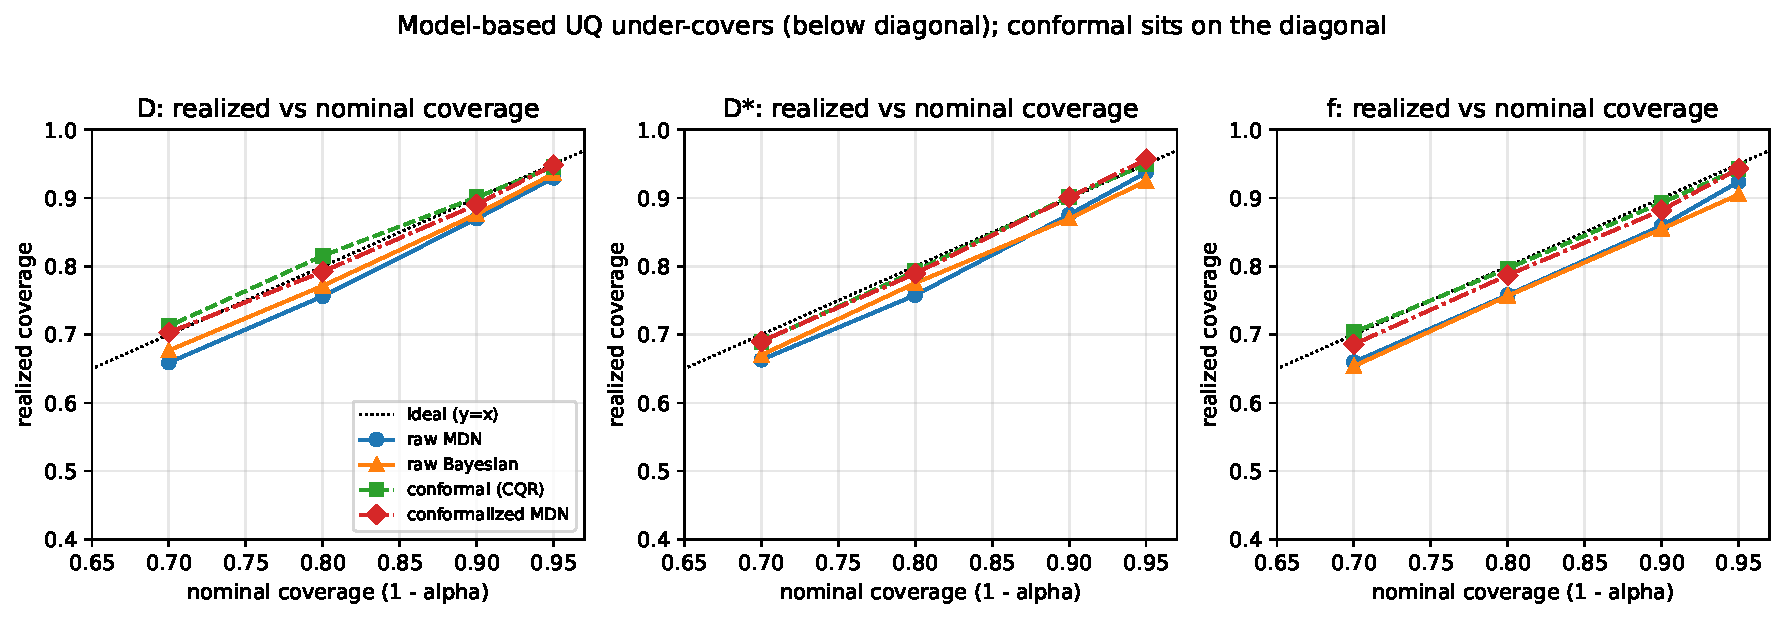
\includegraphics[width=0.78\linewidth]{figures/coverage_vs_nominal.pdf}
\caption{Realized vs nominal coverage per parameter. Raw model-based methods sit
below the diagonal (overconfident); conformal and conformalized methods sit on it.}
\label{fig:coverage}
\end{figure}

\begin{figure}[t]
\centering
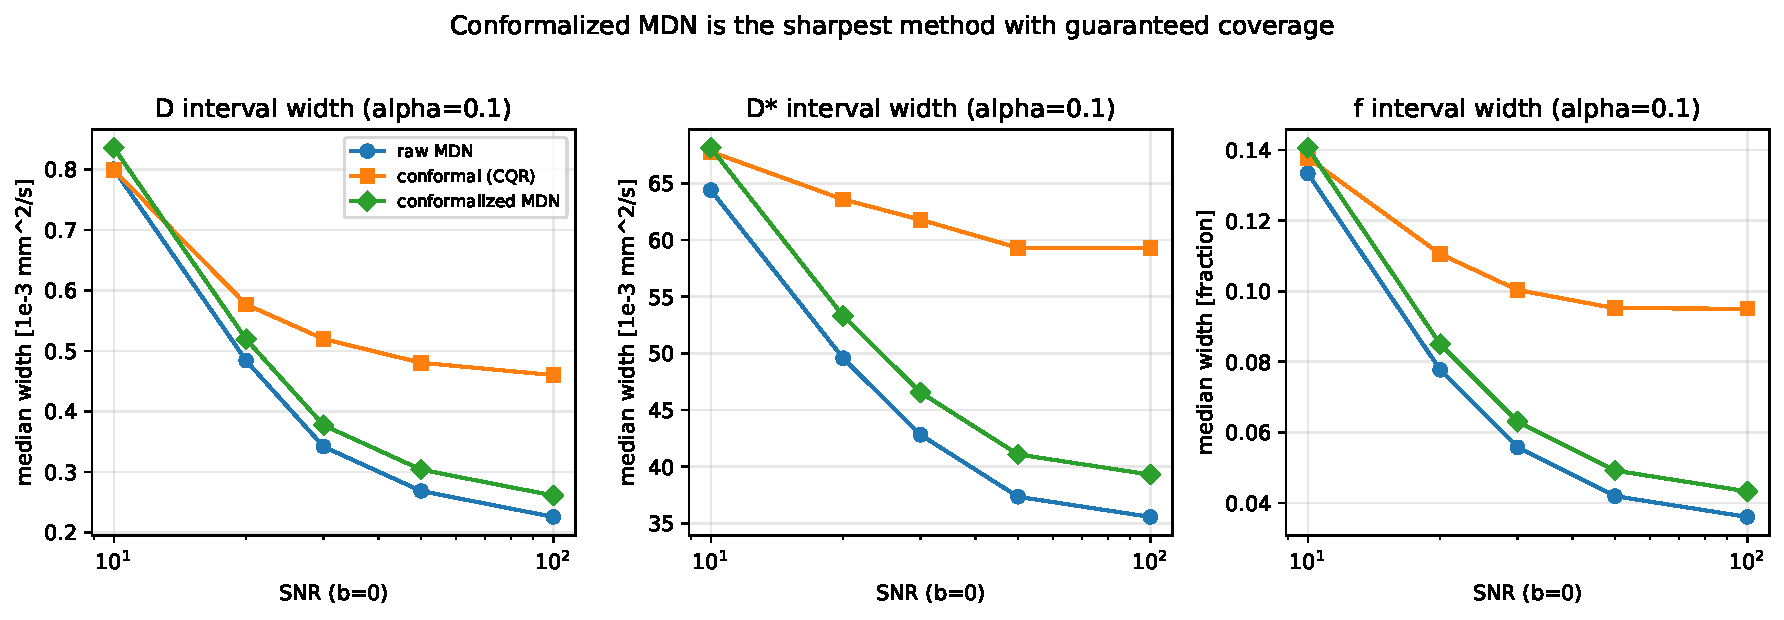
\includegraphics[width=0.78\linewidth]{figures/sharpness_vs_snr.pdf}
\caption{Median interval width vs SNR. Conformalized-MDN is the sharpest method
with a guaranteed coverage level.}
\label{fig:sharpness}
\end{figure}

\subsection{The conditional finding: high-$\Dstar$ under-covers universally}
\label{sec:conditional}
Marginal coverage hides a compartment-specific failure
(Fig.~\ref{fig:heatmap}). On the (SNR $\times$ $\Dstar$-tercile) grid, the
high-$\Dstar$ tercile under-covers for \emph{every} method at \emph{every} SNR,
while the mid-$\Dstar$ tercile over-covers ($\approx0.99$). Table~\ref{tab:hidstar}
gives the high-$\Dstar$ slice: even the best method (conformalized-MDN) reaches
only $0.877$ marginal-in-regime and $0.808$ in its worst-SNR cell. Critically,
\emph{Mondrian stratification by the known SNR does not fix it} -- the failure axis
is the \emph{unknown} true $\Dstar$, not SNR. This is the refined, IVIM-specific
form of the original hypothesis.

\begin{table}[t]
\centering
\caption{High-$\Dstar$ tercile coverage ($\Dstar$ parameter, nominal $0.90$). Every
method under-covers; SNR-Mondrian does not close it. From
\texttt{results/conditional\_report.txt}.}
\label{tab:hidstar}
\small
\begin{tabular}{lcc}
\toprule
arm & hi-$\Dstar$ marginal & hi-$\Dstar$ worst-SNR cell \\
\midrule
raw-MDN              & 0.825 & 0.756 \\
CQR (plain)          & 0.819 & 0.767 \\
split (Mondrian/SNR) & 0.808 & 0.764 \\
CQR (Mondrian/SNR)   & 0.814 & 0.766 \\
conformalized-MDN    & \textbf{0.877} & \textbf{0.808} \\
\bottomrule
\end{tabular}
\end{table}

\begin{figure}[t]
\centering
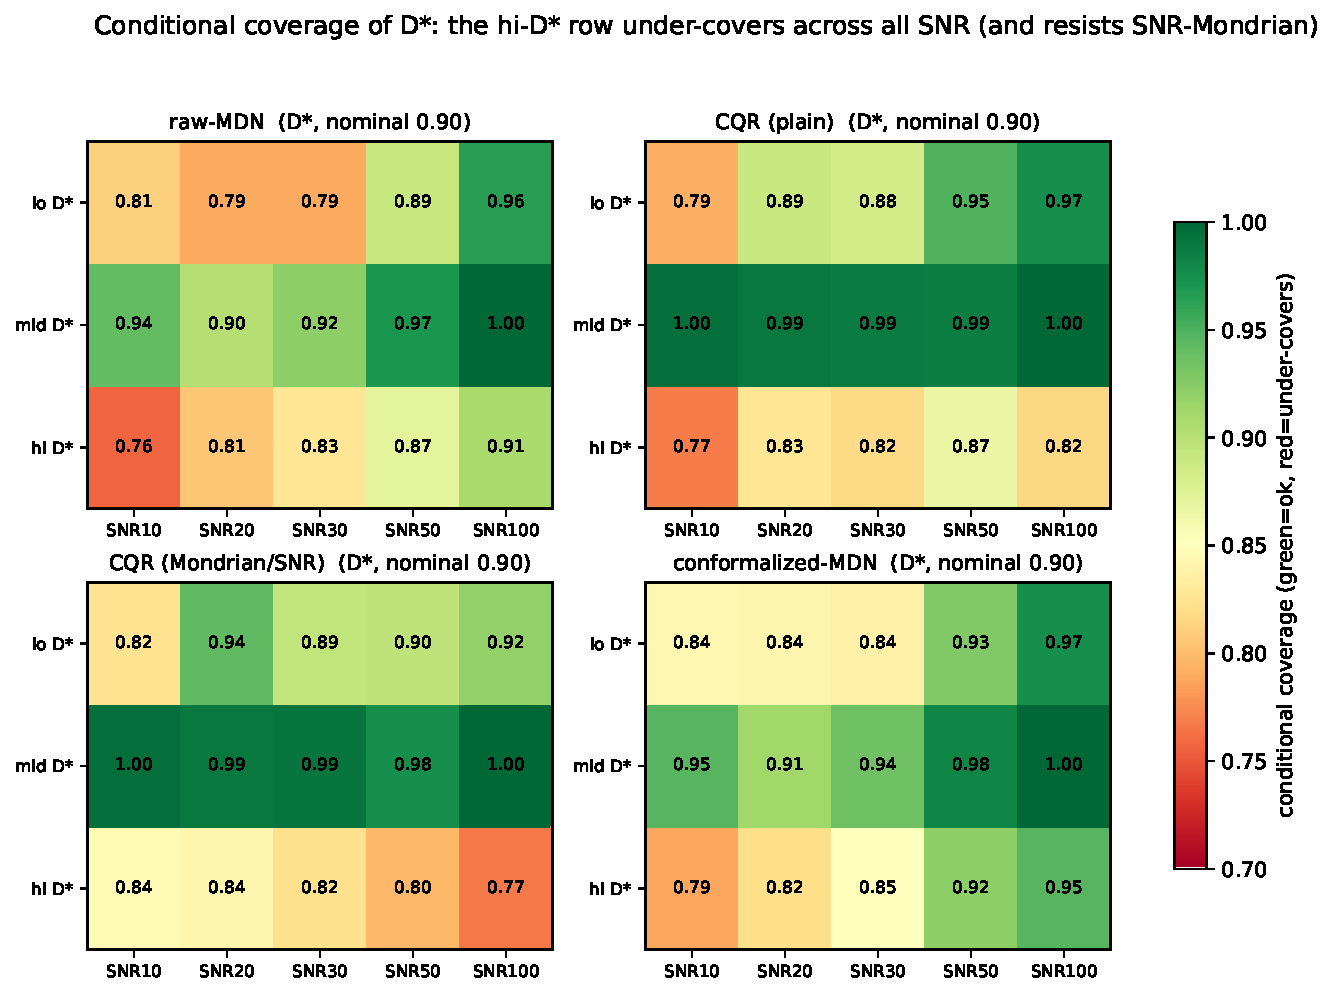
\includegraphics[width=0.72\linewidth]{figures/conditional_coverage_heatmap.pdf}
\caption{SNR $\times$ $\Dstar$-regime conditional coverage. The high-$\Dstar$ row
under-covers across all SNR and resists SNR-Mondrian.}
\label{fig:heatmap}
\end{figure}

\subsection{The high-$\Dstar$ gap is an irreducible identifiability limit}
\label{sec:identifiability}
We attacked the high-$\Dstar$ gap with eleven \emph{label-free} conditioning
methods -- plug-in Mondrian by estimated $\hat{\Dstar}$, localized conformal on
observable features~\citep{guan2023}, and conditional conformal over an observable
basis~\citep{gibbs2023} -- none of which uses the true $\Dstar$
(Fig.~\ref{fig:attack}). \emph{None materially closes the gap.} The best label-free
method (MDN with localized conformal) reaches $0.868$ marginal / $0.819$ worst-SNR,
within sampling noise of the $0.808$ baseline. The reason is structural, not
methodological:
\begin{itemize}
\item \textbf{Routing error.} A plug-in $\hat{\Dstar}$ misroutes $31\%$ of true
high-$\Dstar$ voxels to a lower-$\Dstar$ (smaller-radius) stratum: the estimate is
least reliable exactly where it must route correctly. Mondrian-by-$\hat{\Dstar}$
attains nominal coverage \emph{conditional on the observed stratum}
($[0.90,0.89,0.90]$) yet craters on the \emph{true} high-$\Dstar$ tercile
($0.76$) -- it controls the observable, not the latent axis.
\item \textbf{The CRLB wall.} The CRLB on $\Dstar$ grows $\sim6\times$ from low to
high $\Dstar$; the ratio of median CRLB($\Dstar$) to the tercile bin width rises
$0.34\to0.69\to1.12$ across terciles (Fig.~\ref{fig:crlb}). In the high-$\Dstar$
regime the CRLB \emph{exceeds} the bin width: a voxel's $\Dstar$ cannot be
localized to its own tercile from the data, so no observable can route it to a
wider-interval stratum. Conformal interval width correctly tracks the per-voxel
CRLB (log--log $r=0.75$): the intervals are honest, not broken.
\end{itemize}
\textbf{Verdict.} High-$\Dstar$ regime-conditional coverage in IVIM is an
\emph{irreducible identifiability limit}. We therefore \emph{characterize} the
limit; we do not claim to solve it.

\begin{figure}[t]
\centering

\includegraphics[width=0.82\linewidth]{figures/highdstar_attack.pdf}
\caption{High-$\Dstar$ coverage (marginal and worst-SNR cell) for eleven label-free
conditioning methods; every bar sits below the nominal $0.90$.}
\label{fig:attack}
\end{figure}

\begin{figure}[t]
\centering

\includegraphics[width=0.92\linewidth]{figures/crlb_identifiability.pdf}
\caption{(Left) absolute CRLB($\Dstar$) balloons across the $\Dstar$ range per SNR
(high-$\Dstar$ tercile shaded). (Right) conformal width vs per-voxel CRLB
($r=0.75$): the intervals widen honestly where $\Dstar$ is under-identified.}
\label{fig:crlb}
\end{figure}

\subsection{Robustness under deliberate exchangeability breaks}
\label{sec:robustness}
We deploy one conformal predictor and one monitor, calibrated on the i.i.d.\ Rician
cohort, against four deliberate breaks (Table~\ref{tab:shift},
Fig.~\ref{fig:shift}). Every break miscalibrates coverage; the dangerous
under-coverage reaches $\Dstar=0.515$ under a harder-tissue prior shift and the
worst parameter $0.610$ under a low-SNR covariate shift. \emph{Weighted /
nonexchangeable conformal}~\citep{tibshirani2019,barber2023} cleanly recovers the
covariate shifts (SNR worst-parameter $0.610\to0.899$, all within $0.011$ of
nominal; prior $\Dstar$ $0.515\to0.975$) and is honestly limited on the
tri-exponential forward-model misspecification: a shift in the conditional law
$P(y\mid x)$ is, in general, not repairable by an $x$-space likelihood ratio
(weighting over-corrects $\Dstar$ to $0.928$, leaving a per-parameter spread of
$0.028$).

\begin{table}[t]
\centering
\caption{Per-parameter coverage under each break, naive vs.\ weighted conformal
($\alpha=0.10$, nominal $0.90$), with the deployment monitor's verdict. From
\texttt{results/robustness\_report.txt}.}
\label{tab:shift}
\small
\begin{tabular}{llccc l}
\toprule
scenario & method & $D$ & $\Dstar$ & $f$ & monitor \\
\midrule
in-dist (control)   & naive    & 0.909 & 0.900 & 0.902 & silent (AUC 0.50) \\
SNR shift (low)      & naive    & \textbf{0.610} & 0.744 & \textbf{0.616} & FIRES (AUC 0.91) \\
                     & weighted & 0.901 & 0.899 & 0.911 & \\
prior shift (harder) & naive    & 0.970 & \textbf{0.515} & 0.906 & FIRES (AUC 0.71) \\
                     & weighted & 0.900 & 0.975 & 0.916 & \\
tri-exp misspec      & naive    & 0.908 & 0.846 & 0.910 & FIRES (AUC 0.51) \\
                     & weighted & 0.886 & 0.928 & 0.894 & \\
noise-model swap     & naive    & 0.918 & 0.901 & 0.904 & FIRES (AUC 0.52) \\
\bottomrule
\end{tabular}
\end{table}

The label-free monitor (reusing the deployment-validity concept of a sibling
project) \textbf{fires on all four observable breaks before coverage fails}: in an
SNR-severity sweep, it raises the alarm at SNR $20$ (coverage still $0.866$) while
coverage first crosses the failure line at SNR $13$. Yet it is constitutively
\emph{blind} to the latent high-$\Dstar$ gap: on an in-distribution (exchangeable)
test the monitor is silent (AUC $0.50$) and marginal $\Dstar$ coverage is nominal
($0.900$), while the high-$\Dstar$ conditional coverage is $0.815$. Observable
shifts are caught; the within-distribution latent-axis failure is not -- the same
observable-vs-hidden split that recurs across this line of work.

\begin{figure}[t]
\centering
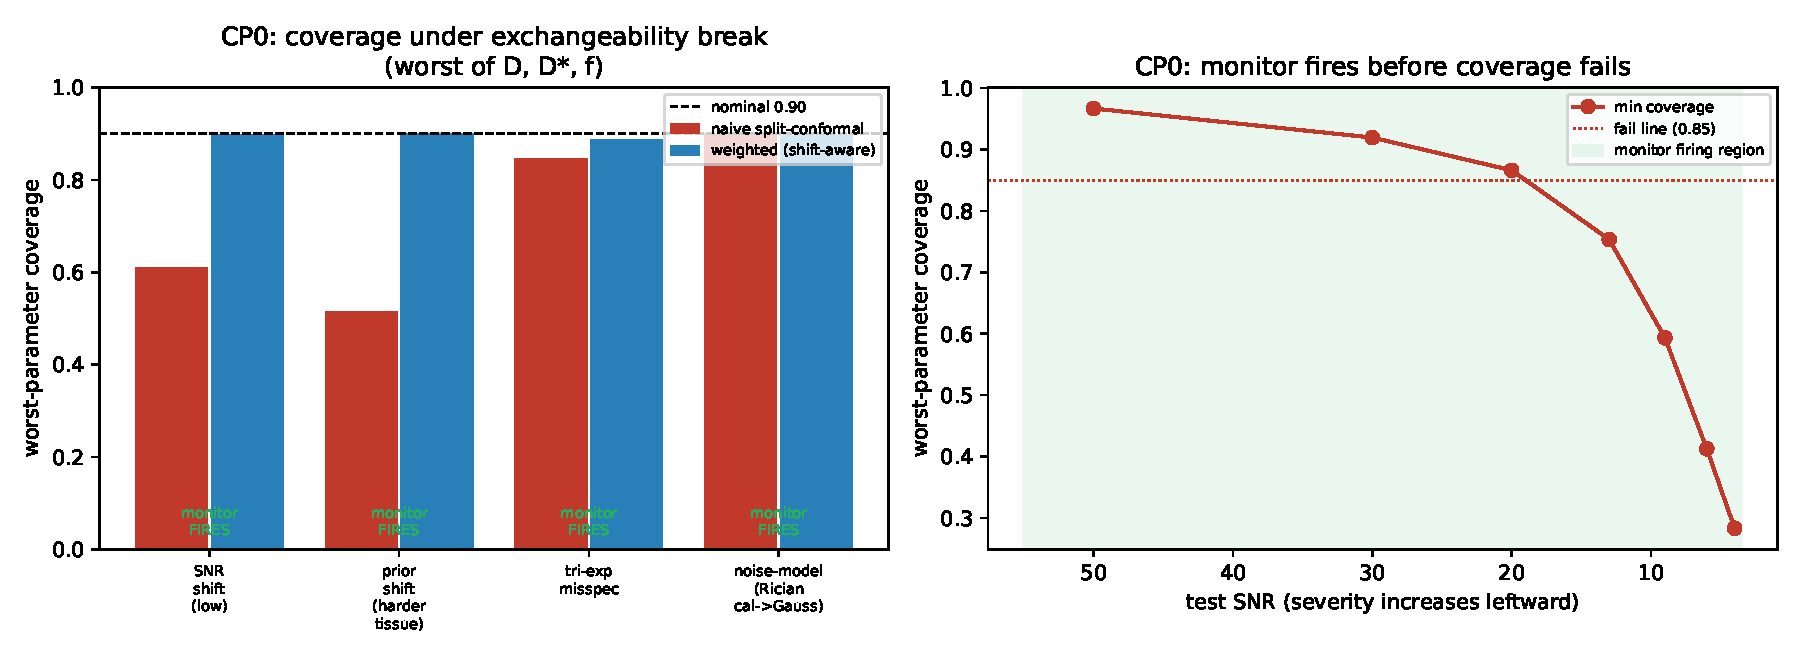
\includegraphics[width=0.92\linewidth]{figures/robustness_shift.pdf}
\caption{(Left) worst-parameter coverage under each exchangeability break, naive
vs.\ weighted, with monitor status. (Right) SNR-severity sweep: the monitor fires
before coverage crosses the failure line.}
\label{fig:shift}
\end{figure}

\subsection{Acquisition sensitivity: the wall is b-scheme-robust}
\label{sec:acquisition}
Does the high-$\Dstar$ wall move with the b-value scheme? We compare a clinical
($11$-value), a CRLB-optimal ($11$-value, greedy $\Dstar$-CRLB design), and a dense
($22$-value) scheme at fixed prior/SNR/seed (Table~\ref{tab:acq},
Fig.~\ref{fig:acq}). The high-$\Dstar$ marginal coverage barely moves
($0.841\to0.844\to0.845$) and the resolution ratio CRLB($\Dstar$)/tercile-width
stays $\ge1.05$ for \emph{every} scheme. A CRLB-optimal design lowers the absolute
CRLB ($1.25\to1.05$) but does not remove the wall. Acquisition design \emph{shifts}
the wall; it does not erase it -- a concrete, honestly negative handoff to
acquisition-aware experiment design.

\begin{table}[t]
\centering
\caption{High-$\Dstar$ coverage and resolution ratio by b-value scheme. From
\texttt{results/robustness\_report.txt}.}
\label{tab:acq}
\small
\begin{tabular}{lcccc}
\toprule
scheme & $n_b$ & hi-$\Dstar$ marg & hi-$\Dstar$ worst-SNR & CRLB/tercile-width \\
\midrule
clinical      & 11 & 0.841 & 0.595 & 1.25 \\
CRLB-optimal  & 11 & 0.844 & 0.608 & \textbf{1.05} \\
dense         & 22 & 0.845 & 0.596 & 1.06 \\
\bottomrule
\end{tabular}
\end{table}

\begin{figure}[t]
\centering
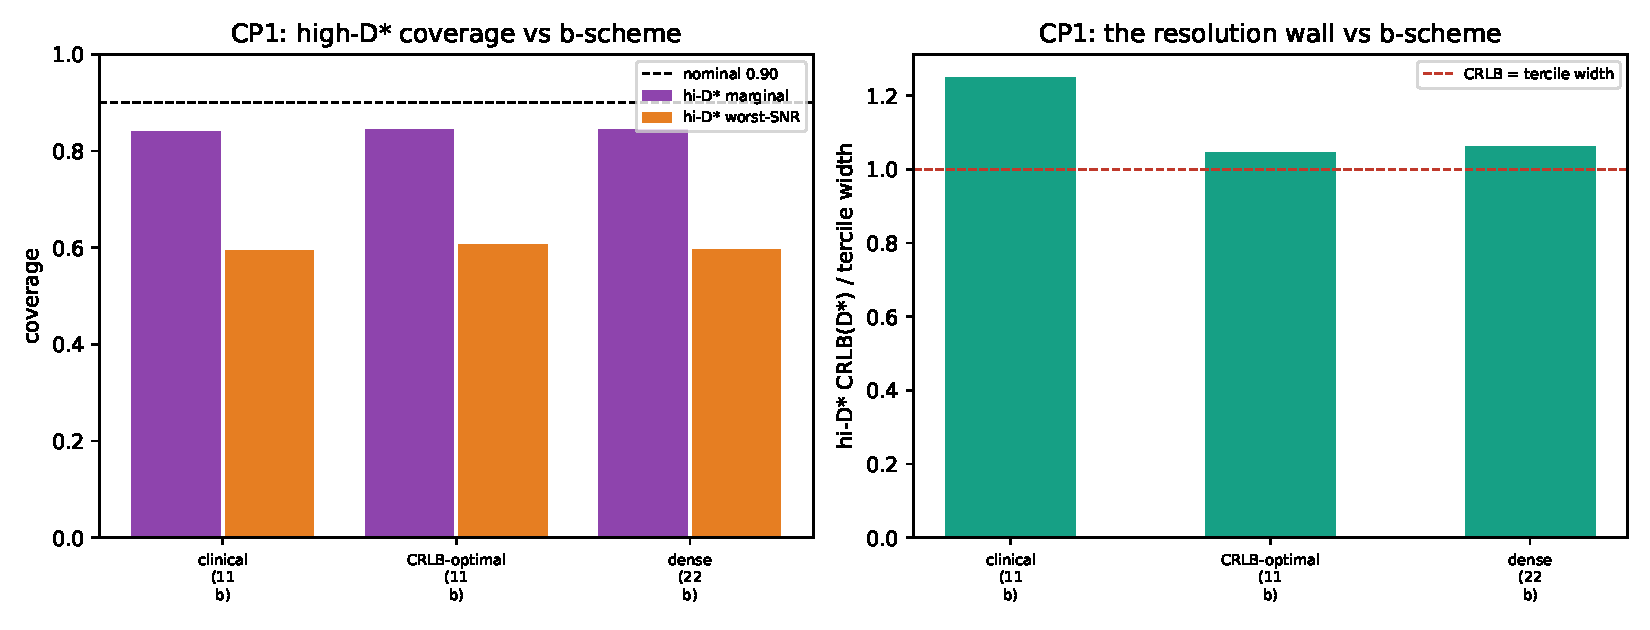
\includegraphics[width=0.92\linewidth]{figures/acquisition_wall.pdf}
\caption{(Left) high-$\Dstar$ coverage vs.\ b-scheme. (Right) the resolution ratio
CRLB($\Dstar$)/tercile-width stays $\ge1$ for every scheme: the regime is
unresolvable regardless of acquisition.}
\label{fig:acq}
\end{figure}

\subsection{In-vivo: a qualitative demonstration, no coverage claim}
\label{sec:invivo}
In vivo there are no ground-truth parameters, so realized coverage is
\emph{unmeasurable} and the finite-sample guarantee is \emph{not asserted}. We
demonstrate the deployed pipeline qualitatively (Fig.~\ref{fig:invivo}): the
conformalized $\Dstar$ band widths are wide and heavy-tailed ($10/50/90$th
percentile $=47/64/79\times10^{-3}\unit{mm^2/s}$; widest-to-narrowest decile ratio
$1.7\times$), ballooning on voxels where the perfusion compartment is
under-identified -- the wall, now on signal. Pointed at the deployment data with a
synthetic calibration, the deployment monitor \textbf{fires} (AUC $0.84$):
synthetic$\to$deployment is itself a large exchangeability break, and the monitor
detects it. That firing is the honest, label-free reason the synthetic guarantee
must not be transferred in vivo without re-calibration on matched labeled data --
which in vivo does not exist. The monitor turns ``no ground truth'' into an
observable stop sign. (No usable permissively-licensed, ground-truth-free in-vivo
IVIM dataset was available for this study; the demonstration runs on a clearly
labeled synthetic stand-in, and dataset choice/licensing and the in-vivo framing
are deferred to human sign-off.)

\begin{figure}[t]
\centering
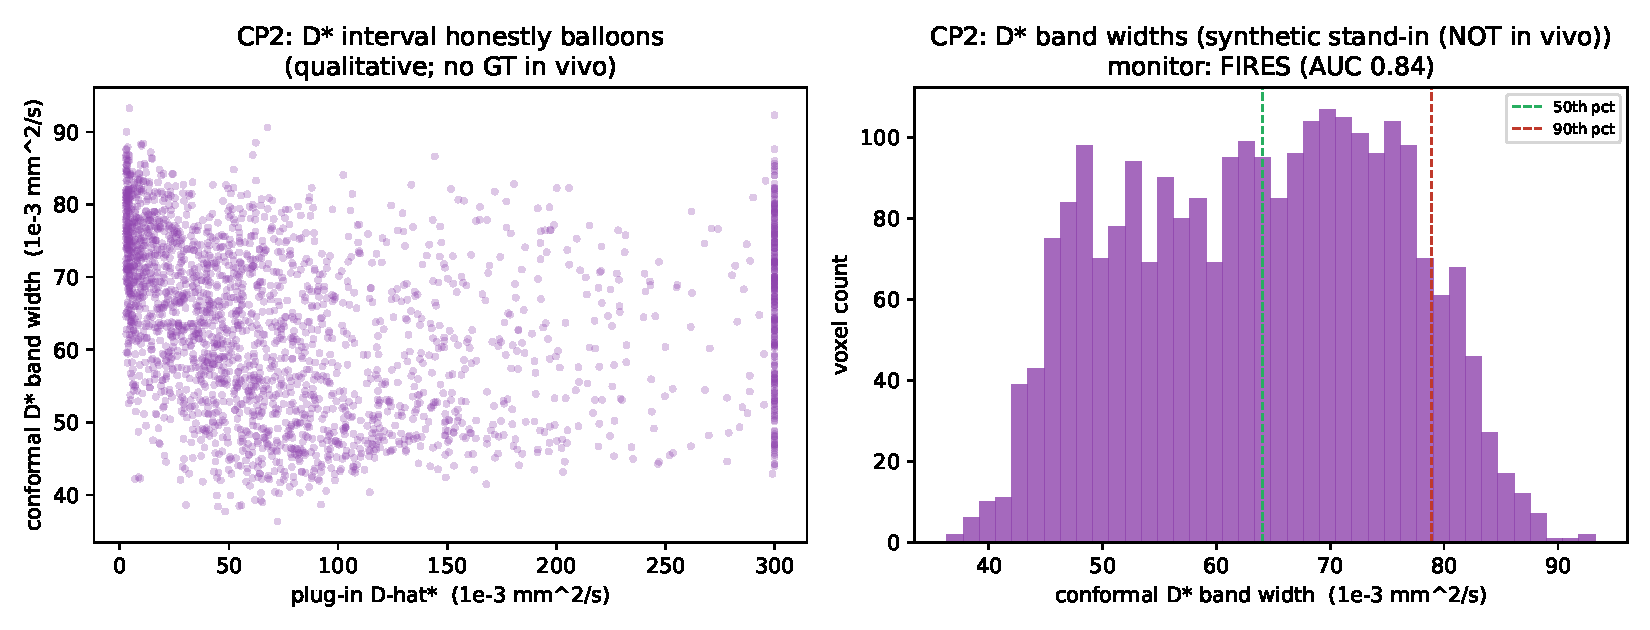
\includegraphics[width=0.92\linewidth]{figures/invivo_demo.pdf}
\caption{In-vivo qualitative demo (synthetic stand-in). (Left) the conformal
$\Dstar$ band balloons with the plug-in $\hat{\Dstar}$. (Right) the heavy-tailed
$\Dstar$ band-width distribution; the deployment monitor fires on the transfer.}
\label{fig:invivo}
\end{figure}

\section{Discussion}
The thread connecting these results is an \emph{observable-vs-latent} distinction.
Conformal prediction guarantees \emph{marginal} coverage and, with weighting or
stratification on \emph{observable} quantities (SNR, signal features, estimated
density ratios), can recover coverage conditional on those observables. What it
cannot label-free-guarantee is coverage conditional on a \emph{latent} axis that
the data do not identify. In IVIM that latent axis is the true $\Dstar$ in its
ill-posed regime: the Fisher information there collapses, the CRLB exceeds the bin
width, and no observable proxy -- including the plug-in $\hat{\Dstar}$ -- recovers
the regime. This is why an observable deployment monitor catches every
\emph{distribution} shift but is blind to the \emph{within-distribution} high-$\Dstar$
gap.

The same wall appears in adjacent label-free problems: deployment-validity
monitoring is provably blind to shifts that leave observable statistics unchanged
(a ``hidden channel''), and the absence of in-vivo ground truth (the ``Echo
tension'') forecloses any direct coverage check on real data. We read these not as
failures of conformal prediction -- whose guarantee is exactly as advertised -- but
as a recurring \emph{identifiability} boundary: distribution-free tools deliver
everything the data identify and nothing they do not. Practically, this argues for
(i) conformalizing a strong model-based base (sharpest valid intervals), (ii)
deploying an observable monitor to guard exchangeability, and (iii) reporting the
high-$\Dstar$ compartment as characterized-but-unresolved rather than trusting a
point map there.

\section{Limitations}
Our coverage results are \emph{synthetic-primary} by necessity: conformal
calibration needs labels that in-vivo IVIM lacks, so the guarantee is established
on a forward model we control, and the in-vivo component is explicitly qualitative
with no coverage claim. The synthetic cohort uses uniform priors over published
ranges and Rician noise; real tissue is more heterogeneous, and the
tri-exponential and prior-shift stresses (Sec.~\ref{sec:robustness}) are
deliberately schematic probes of misspecification rather than a tissue model. The
CRLB diagnostic uses the high-SNR Gaussian approximation to Rician noise; the
qualitative under-identification of $\Dstar$ is noise-model-independent (the
$\Dstar$ Jacobian column vanishes as $\Dstar$ grows), but absolute bound values at
SNR $\lesssim10$ would shift under an exact Rician treatment. Finally, all coverage
guarantees assume exchangeability of calibration and deployment data; the monitor
quantifies, but cannot by itself repair, departures from it.

\section{Consistency check (reproducibility)}
\label{sec:consistency}
Every numeric claim in this manuscript is drawn from a gated, seeded checkpoint
printout across Gauge~01--04. The script \texttt{gauge/paper/consistency.py}
re-reads the committed report files (\texttt{results/*.txt}, \texttt{POSITIONING.md})
and asserts that each headline number used here appears verbatim in its source; it
prints a one-paragraph pass/fail summary. The full pipeline regenerates
deterministically from seed \texttt{20260613} (\texttt{python -m gauge.baselines};
\texttt{gauge.benchmark}; \texttt{gauge.conditional}; \texttt{gauge.conditional\_attack};
\texttt{gauge.robustness}; \texttt{gauge.invivo}).

\section{Conclusion}
Gauge brings distribution-free conformal coverage to the ill-posed IVIM inverse
problem and benchmarks it against model-based UQ. The naive hypothesis -- that the
conformal advantage concentrates marginally in $\Dstar/f$ -- is rejected:
model-based IVIM UQ is overconfident broadly, conformal restores coverage
everywhere, and conformalizing the MDN is the sharpest valid recipe. The genuine
IVIM-specific phenomenon is conditional: the high-$\Dstar$ regime under-covers
universally, and a Fisher-information analysis shows this is an irreducible
identifiability limit that no label-free method can close. We therefore characterize
the limit -- and provide the robustness tooling, acquisition analysis, and
qualitative in-vivo demonstration that frame how an honest, distribution-free IVIM
uncertainty map should be deployed and monitored.

\section*{Data and Code Availability Statement}
This study uses no human or animal data. All results are produced from a
deterministic, seeded synthetic cohort (seed \texttt{20260613}) generated by the
study's own forward model; no external or in-vivo dataset is required to reproduce
them. The complete source code, the gated checkpoint outputs from which every
number in this paper is drawn, the figures, and a machine-checked consistency
script (\texttt{gauge/paper/consistency.py}) are openly available in the project
repository and permanently archived at
\href{https://doi.org/10.5281/zenodo.20686274}{https://doi.org/10.5281/zenodo.20686274}.

\section*{Conflict of Interest}
The author declares no competing interests.

\section*{Funding}
This research received no specific grant from any funding agency in the public,
commercial, or not-for-profit sectors; it was conducted independently by the
author.

\section*{Author Contributions}
Avery Karlin is the sole author and conceived the study, designed and implemented
the methods and software, performed the analysis, produced the figures, and wrote
the manuscript.

\section*{ORCID}
Avery Karlin \quad \href{https://orcid.org/0000-0003-3848-6782}{https://orcid.org/0000-0003-3848-6782}

\bibliographystyle{unsrtnat}
\bibliography{refs}

\end{document}
